\documentclass[a4paper,14pt,oneside,openany]{memoir}

% Setting document margins and spacing
\usepackage[left=30mm, right=15mm, top=20mm, bottom=20mm]{geometry}
\pagestyle{plain}
\parindent=1.25cm
\usepackage{indentfirst}

% Setting language and font
\usepackage[english, russian]{babel}
\usepackage{fontspec}
\setmainfont{Times New Roman}
\setsansfont{Times New Roman}
\setmonofont{Times New Roman}

% Configuring code listings
\usepackage{listings}
\usepackage{xcolor}
\lstset{
	language=Matlab,
	basicstyle=\ttfamily\small,
	keywordstyle=\color{blue}\bfseries,
	commentstyle=\color{gray}\itshape,
	stringstyle=\color{red},
	numbers=left,
	numberstyle=\tiny,
	stepnumber=1,
	numbersep=5pt,
	showspaces=false,
	showstringspaces=false,
	frame=single,
	breaklines=true,
	breakatwhitespace=true,
	tabsize=2
}

% Configuring headings and subheadings
\setsecnumdepth{subsection}
\renewcommand*{\chapterheadstart}{}
\renewcommand*{\printchaptername}{}
\renewcommand*{\chapnumfont}{\normalfont\bfseries}
\renewcommand*{\afterchapternum}{\hspace{1em}}
\renewcommand*{\printchaptertitle}{\normalfont\bfseries\centering\MakeUppercase}
\setbeforesecskip{20pt}
\setaftersecskip{20pt}
\setsecheadstyle{\raggedright\normalfont\bfseries}
\setbeforesubsecskip{20pt}
\setaftersubsecskip{20pt}
\setsubsecheadstyle{\raggedright\normalfont\bfseries}

% Configuring table of contents
\addto\captionsrussian{\renewcommand\contentsname{Содержание}}
\setrmarg{2.55em plus1fil}
\renewcommand{\aftertoctitle}{\afterchaptertitle \vspace{-\cftbeforechapterskip}}
\renewcommand*{\cftchapternumwidth}{1.5em}
\renewcommand*{\cftchapterfont}{\normalfont\MakeUppercase}
\renewcommand*{\cftchapterpagefont}{\normalfont}
\renewcommand*{\cftchapterdotsep}{\cftdotsep}
\renewcommand*{\cftdotsep}{1}
\renewcommand*{\cftchapterleader}{\cftdotfill{\cftchapterdotsep}}
\maxtocdepth{subsection}

% Configuring text alignment and hyphenation
\tolerance 1414
\hbadness 1414
\emergencystretch 1.5em
\hfuzz 0.3pt
\vfuzz \hfuzz
\clubpenalty=10000
\widowpenalty=10000
\brokenpenalty=4991

% Defining Russian alphabet for enumerations
\makeatletter
\def\russian@Alph#1{\ifcase#1\or
	А\or Б\or В\or Г\or Д\or Е\or Ж\or
	И\or К\or Л\or М\or Н\or
	П\or Р\or С\or Т\or У\or Ф\or Х\or
	Ц\or Ш\or Щ\or Э\or Ю\or Я\else\xpg@ill@value{#1}{russian@Alph}\fi}
\def\russian@alph#1{\ifcase#1\or
	а\or б\or в\or г\or д\or е\or ж\or
	и\or к\or л\or м\or н\or
	п\or р\or с\or т\or у\or ф\or х\or
	ц\or ш\or щ\or э\or ю\or я\else\xpg@ill@value{#1}{russian@alph}\fi}
\makeatother

% Configuring figures and subfigures
\usepackage{graphicx, caption, subcaption}
\graphicspath{{images/}}
\captionsetup[figure]{font=small, width=\textwidth, name=Рисунок, justification=centering}
\captionsetup[subfigure]{font=small}
\captiondelim{ --- }
\setkeys{Gin}{width=\textwidth}
\renewcommand{\thesubfigure}{\asbuk{subfigure}}
\usepackage[section]{placeins}

% Configuring hyperlinks
\usepackage{hyperref}
\hypersetup{
	colorlinks=true,
	linktoc=all,
	linktocpage=true,
	linkcolor=red,
	citecolor=red
}

% Configuring lists
\usepackage{enumitem}
\renewcommand*{\labelitemi}{\normalfont{--}}
\makeatletter
\AddEnumerateCounter{\asbuk}{\russian@alph}
\makeatother
\renewcommand{\labelenumii}{\asbuk{enumii})}
\renewcommand{\labelenumiii}{\arabic{enumiii})}
\setlist{noitemsep, leftmargin=*}
\setlist[1]{labelindent=\parindent}
\setlist[2]{leftmargin=\parindent}
\setlist[3]{leftmargin=\parindent}

% Configuring counters
\counterwithout{figure}{chapter}
\counterwithout{equation}{chapter}

% Configuring bibliography
\usepackage{csquotes}
\usepackage[%
backend=biber,
bibencoding=utf8,
sorting=none,
style=gost-numeric,
language=auto,
autolang=other,
sortcites=true,
movenames=false,
maxnames=5,
minnames=3,
doi=false,
isbn=false
]{biblatex}
\DeclareDelimFormat{bibinitdelim}{}

% Inline bibliography
\begin{filecontents*}{biba.bib}
	@book{oppenheim1999,
		Codex: 0,
		title={Discrete-Time Signal Processing},
		author={Oppenheim, Alan V. and Schafer, Ronald W.},
		year={1999},
		publisher={Prentice Hall}
	}
	
	@article{vanNee2000,
		Codex: 0,
		title={OFDM for Wireless Multimedia Communications},
		author={Van Nee, Richard and Prasad, Ramjee},
		journal={Artech House},
		year={2000}
	}
\end{filecontents*}
\addbibresource{biba.bib}

\DeclareSourcemap{
	\maps[datatype=bibtex]{
		\map{
			\step[fieldsource=title, match=\regexp{^\P{Cyrillic}*\p{Cyrillic}.*}, final]
			\step[fieldset=langid, fieldvalue={russian}]
		}
		\map{
			\step[fieldset=langid, fieldvalue={english}]
		}
	}
}

% Additional packages
\usepackage{longtable,ltcaption}
\usepackage{multirow,makecell}
\usepackage{booktabs}
\usepackage{soulutf8}
\usepackage{icomma}
\usepackage{hyphenat}
\usepackage{textcomp}
\usepackage[version=4]{mhchem}
\usepackage{amsmath}

\begin{document}
	
	% Title page
	\thispagestyle{empty}
	
	\begin{center}
		МИНИСТЕРСТВО ЦИФРОВОГО РАЗВИТИЯ, СВЯЗИ И МАССОВЫХ КОММУНИКАЦИЙ \\ РОССИЙСКОЙ ФЕДЕРАЦИИ
		
		\vspace{20pt}
		
		Федеральное государственное бюджетное образовательное учреждение  \\  высшего образования \\
		``Сибирский государственный университет телекоммуникаций и информатики'' \\
		
		\vspace{20pt}
		
		Кафедра телекоммуникационных систем и вычислительных средств \\  (ТС и ВС)
	\end{center}
	
	\vfill
	
	\begin{center}
		РЕФЕРАТ \\  
		по дисциплине \\
		\textit{``Моделирование систем мобильной связи''}
		
		\vspace{20pt}
		
		по теме: \\
		\uppercase{Обработка сигнала в OFDM системе}
	\end{center}
	
	\vfill
	
	\noindent Студент: \\
	\textit{Группа № xxxx \hfill Н. Е. Ляпин}
	
	\vspace{20pt}
	
	\noindent Преподаватель: \\
	\textit{доцент, к.т.н. \hfill Р. В. Ахпашев}
	
	\vfill
	
	\begin{center}
		Новосибирск 2025 г.
	\end{center}
	
	% Setting page numbering and spacing
	\newpage
	\setcounter{page}{2}
	\OnehalfSpacing*
	
	% Table of contents
	\tableofcontents*
	
	% Introduction
	\chapter*{ВВЕДЕНИЕ}
	
	Система с ортогональным частотным разделением каналов (OFDM, Orthogonal Frequency Division Multiplexing) --- это метод модуляции, широко используемый в современных системах связи, таких как Wi-Fi, LTE и DVB-T \cite{vanNee2000}. Благодаря использованию ортогональных поднесущих, OFDM обеспечивает высокую устойчивость к многолучевому распространению сигнала и эффективное использование частотного спектра.
	
	Цель данного проекта --- реализация и анализ полного цикла обработки сигнала в OFDM системе с использованием MATLAB. Проект включает кодирование текстового сообщения, модуляцию, передачу через моделируемый многолучевой канал с аддитивным белым гауссовым шумом (AWGN), демодуляцию и декодирование. Отчет описывает теоретические основы, этапы обработки сигнала, результаты моделирования и анализ качества передачи.
	
	% Chapter 1: Theoretical Foundations
	\chapter{ТЕОРЕТИЧЕСКИЕ ОСНОВЫ OFDM}
	
	\section{Принципы OFDM}
	
	OFDM основан на разделении широкополосного сигнала на множество узкополосных поднесущих, которые ортогональны друг другу. Это позволяет минимизировать межсимвольную интерференцию. На стороне передатчика данные преобразуются с помощью обратного быстрого преобразования Фурье (IFFT), а на стороне приемника --- с помощью прямого быстрого преобразования Фурье (FFT). Добавление циклического префикса (CP) помогает устранить эффекты многолучевого распространения \cite{oppenheim1999}.
	
	\section{Кодирование и модуляция}
	
	Процесс передачи данных включает несколько этапов:
	\begin{itemize}
		\item \textbf{Знаковое кодирование}: преобразование текста в битовую последовательность с использованием заданного алфавита.
		\item \textbf{Сверточное кодирование}: повышение устойчивости к ошибкам с помощью сверточного кода.
		\item \textbf{Перемежка}: случайное перераспределение битов для защиты от пакетных ошибок.
		\item \textbf{QPSK модуляция}: преобразование бит в комплексные символы с использованием квадратурной фазовой манипуляции.
	\end{itemize}
	
	\section{Эффекты канала}
	
	Канал передачи моделируется с учетом многолучевого распространения, где сигнал приходит по нескольким путям с разными задержками и затуханиями. Добавление AWGN имитирует шум реальных систем связи.
	
	% Chapter 2: Signal Processing in OFDM Systems
	\chapter{ОБРАБОТКА СИГНАЛА В OFDM СИСТЕМАХ}
	
	\section{Обработка на стороне передатчика}
	
	Передатчик выполняет следующие шаги:
	\begin{itemize}
		\item Знаковое кодирование текста в биты с использованием алфавита, включающего буквы, цифры, пробел и точку.
		\item Сверточное кодирование с длиной ограничения 7 и генераторными полиномами [171, 133].
		\item Перемежка для защиты от пакетных ошибок.
		\item QPSK модуляция, преобразующая пары бит в комплексные символы.
		\item OFDM модуляция с использованием 64 поднесущих и циклического префикса.
	\end{itemize}
	
	\section{Моделирование канала}
	
	Канал моделируется как многолучевой с 7 лучами, случайными задержками и затуханиями. Мощность шума задается параметром \texttt{noisePowerBW} = -120 дБ. Полоса пропускания канала составляет 13 МГц, а несущая частота --- 1.9 ГГц.
	
	\section{Обработка на стороне приемника}
	
	Приемник выполняет обратные операции:
	\begin{itemize}
		\item OFDM демодуляция с удалением циклического префикса и применением FFT.
		\item QPSK демодуляция для преобразования комплексных символов в биты.
		\item Деперемежка для восстановления исходного порядка бит.
		\item Декодирование Витерби для исправления ошибок.
		\item Знаковое декодирование для получения исходного текста.
	\end{itemize}
	
	\section{Описание функций MATLAB}
	
	Для реализации OFDM-системы использовались функции MATLAB, обеспечивающие кодирование, модуляцию, моделирование канала и обработку сигнала. Ниже приведено подробное описание каждой функции с примерами кода.
	
	\subsection{Функция \texttt{calculateBER}}
	Вычисляет коэффициент битовых ошибок (BER) между исходной и декодированной последовательностью.
	
	\begin{lstlisting}
		originalBits = [1 0 1 1 0];
		decodedBits = [1 0 0 1 1];
		ber = calculateBER(originalBits, decodedBits);
	\end{lstlisting}
	
	Функция сравнивает биты и делит количество ошибок на длину последовательности.
	
	\subsection{Функция \texttt{channel\_config}}
	Возвращает структуру с параметрами канала: 7 лучей, шум -120 дБ, полоса 13 МГц, несущая частота 1.9 ГГц.
	
	\begin{lstlisting}
		params = channel_config();
	\end{lstlisting}
	
	\subsection{Функция \texttt{convolutionalEncoder}}
	Выполняет сверточное кодирование с треллисом (длина ограничения 7, полиномы [171, 133]).
	
	\begin{lstlisting}
		inputBits = [1 0 1];
		encodedBits = convolutionalEncoder(inputBits);
	\end{lstlisting}
	
	\subsection{Функция \texttt{deinterleaver}}
	Восстанавливает порядок бит, используя сохранённый вектор перестановки.
	
	\begin{lstlisting}
		setappdata(0, 'permutationVector', [2 1 3]);
		inputBits = [0 1 1];
		deinterleavedBits = deinterleaver(inputBits);
		disp(deinterleavedBits); % [1 0 1]
	\end{lstlisting}
	
	\subsection{Функция \texttt{getAlphabet}}
	Возвращает алфавит (63 символа) и количество бит на символ (6).
	
	\begin{lstlisting}
		[alphabet, bitPerSymbol] = getAlphabet();
		disp(bitPerSymbol); % 6
	\end{lstlisting}
	
	\subsection{Функция \texttt{getCodingParameters}}
	Возвращает параметры кодирования: длина ограничения 7, полиномы [171, 133].
	
	\begin{lstlisting}
		[constraintLength, codeGenerator] = getCodingParameters();
		disp(codeGenerator); % [171 133]
	\end{lstlisting}
	
	\subsection{Функция \texttt{interleaver}}
	Перемешивает биты для защиты от ошибок, сохраняя перестановку.
	
	\begin{lstlisting}
		inputbits = [1 0 1 1];
		interleavedBits = interleaver(inputbits);
	\end{lstlisting}
	
	\subsection{Функция \texttt{multipathChannel}}
	Моделирует многолучевой канал с 7 лучами и AWGN.
	
	\begin{lstlisting}
		params = channel_config();
		txSignal = randn(1, 100);
		receivedSignal = multipathChannel(txSignal, params);
		disp(length(receivedSignal)); % 100
	\end{lstlisting}
	
	\subsection{Функция \texttt{ofdm\_config}}
	Задаёт параметры OFDM: 64 поднесущие, циклический префикс 1/16.
	
	\begin{lstlisting}
		params = ofdm_config();
		disp(params.cpLength); % 4
	\end{lstlisting}
	
	\subsection{Функция \texttt{ofdmDemodulator}}
	Выполняет OFDM-демодуляцию, извлекая QPSK-символы.
	
	\begin{lstlisting}
		setappdata(0, 'cpLength', 4);
		receivedSignal = randn(68, 1);
		qpskSymbols = ofdmDemodulator(receivedSignal);
		disp(length(qpskSymbols)); % 64
	\end{lstlisting}
	
	\subsection{Функция \texttt{ofdmModulator}}
	Выполняет OFDM-модуляцию с циклическим префиксом.
	
	\begin{lstlisting}
		params = ofdm_config();
		qpskSymbols = randn(64, 1);
		ofdm_stream = ofdmModulator(qpskSymbols, params);
		disp(length(ofdm_stream)); % 68
	\end{lstlisting}
	
	\subsection{Функция \texttt{qpskDemodulator}}
	Демодулирует QPSK-символы в биты по квадрантам.
	
	\begin{lstlisting}
		receivedSymbols = [0.707+0.707j, -0.707-0.707j];
		demodulatedBits = qpskDemodulator(receivedSymbols);
		disp(demodulatedBits); % [0 0 1 1]
	\end{lstlisting}
	
	\subsection{Функция \texttt{qpskModulator}}
	Модулирует биты в QPSK-символы.
	
	\begin{lstlisting}
		inputBits = [0 0 1 1];
		modulatedSymbols = qpskModulator(inputBits);
		disp(modulatedSymbols); % [0.707+0.707j -0.707-0.707j]
	\end{lstlisting}
	
	\subsection{Функция \texttt{symbolDecoder}}
	Декодирует биты в текстовое сообщение.
	
	\begin{lstlisting}
		encodedBits = [0 0 0 0 1 0];
		decodedMessage = symbolDecoder(encodedBits);
		disp(decodedMessage); % 'b'
	\end{lstlisting}
	
	\subsection{Функция \texttt{symbolEncoder}}
	Кодирует текст в биты.
	
	\begin{lstlisting}
		message = 'b';
		encodedBits = symbolEncoder(message);
		disp(encodedBits); % [0 0 0 0 1 0]
	\end{lstlisting}
	
	\subsection{Функция \texttt{viterbiDecoder}}
	Выполняет декодирование Витерби.
	
	\begin{lstlisting}
		encodedBits = [1 1 0 1 0 0];
		decodedBits = viterbiDecoder(encodedBits);
	\end{lstlisting}
	
	% Chapter 3: Simulation and Results
	\chapter{МОДЕЛИРОВАНИЕ И РЕЗУЛЬТАТЫ}
	
	\section{Настройка моделирования}
	
	Моделирование проводилось с использованием следующих параметров:
	\begin{itemize}
		\item Количество поднесущих: 64;
		\item Длина циклического префикса: 1/16 от числа поднесущих;
		\item Тип модуляции: QPSK;
		\item Количество лучей в канале: 7;
		\item Полоса пропускания: 13 МГц.
	\end{itemize}
	
	Тестовое сообщение: \texttt{\mbox{HELLO WORLD THIS IS A TEST MESSAGE.}}
	
	\section{Результаты и анализ}
	
	Моделирование показало успешное восстановление тестового сообщения. Основные результаты:
	\begin{itemize}
		\item Спектр переданного OFDM символа демонстрирует равномерное распределение энергии по поднесущим (см. рисунок \ref{fig:signal_analysis}\subref{fig:signal_analysis:a}).
		\item Спектр до эквалайзирования показывает искажения, вызванные каналом (см. рисунок \ref{fig:signal_analysis}\subref{fig:signal_analysis:b}).
		\item Созвездие QPSK в передатчике имеет четкие точки, соответствующие четырем фазам, тогда как в приемнике наблюдается шум (см. рисунок \ref{fig:signal_analysis}\subref{fig:signal_analysis:c}, \subref{fig:signal_analysis:d}).
		\item Коэффициент битовых ошибок (BER) до знакового декодирования составил $10^{-3}$, что указывает на высокую точность передачи.
	\end{itemize}
	
	\begin{figure}[ht]
		\centering
		\begin{subfigure}{0.45\textwidth}
			\centering
			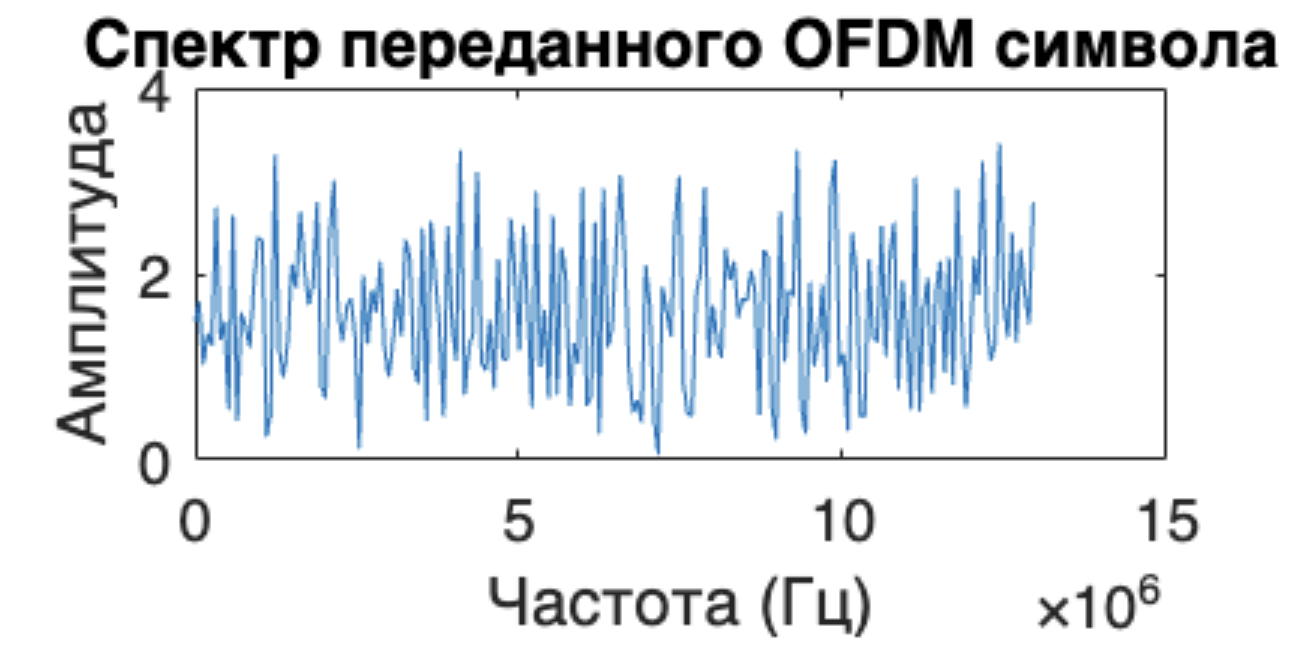
\includegraphics{ofdm_spectrum_tx.png}
			\caption{Спектр переданного OFDM символа}
			\label{fig:signal_analysis:a}
		\end{subfigure}
		\hfill
		\begin{subfigure}{0.45\textwidth}
			\centering
			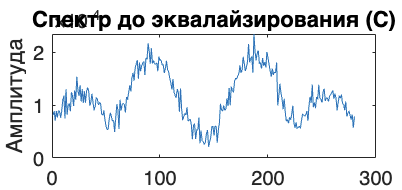
\includegraphics{spectrum_before_eq.png}
			\caption{Спектр до эквалайзирования}
			\label{fig:signal_analysis:b}
		\end{subfigure}
		\hfill
		\begin{subfigure}{0.45\textwidth}
			\centering
			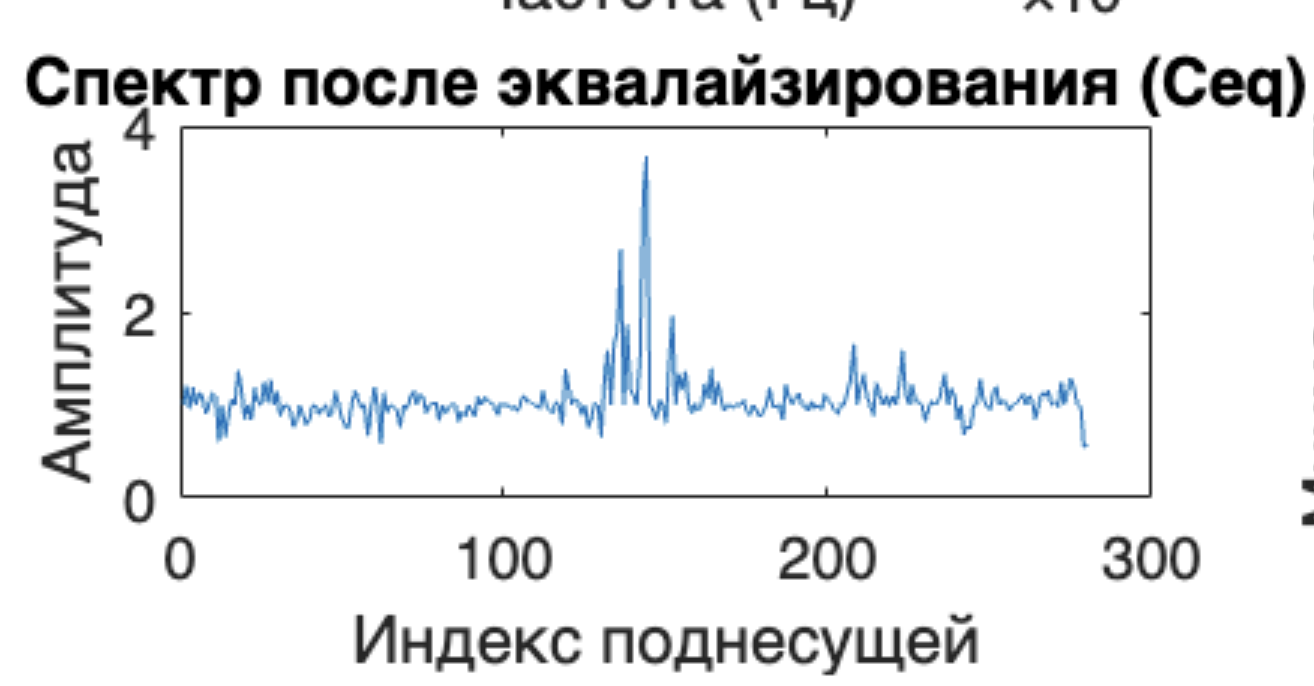
\includegraphics{spectrum_after_eq.png}
			\caption{Спектр после эквалайзирования}
			\label{fig:signal_analysis:c}
		\end{subfigure}
		\begin{subfigure}{0.45\textwidth}
			\centering
			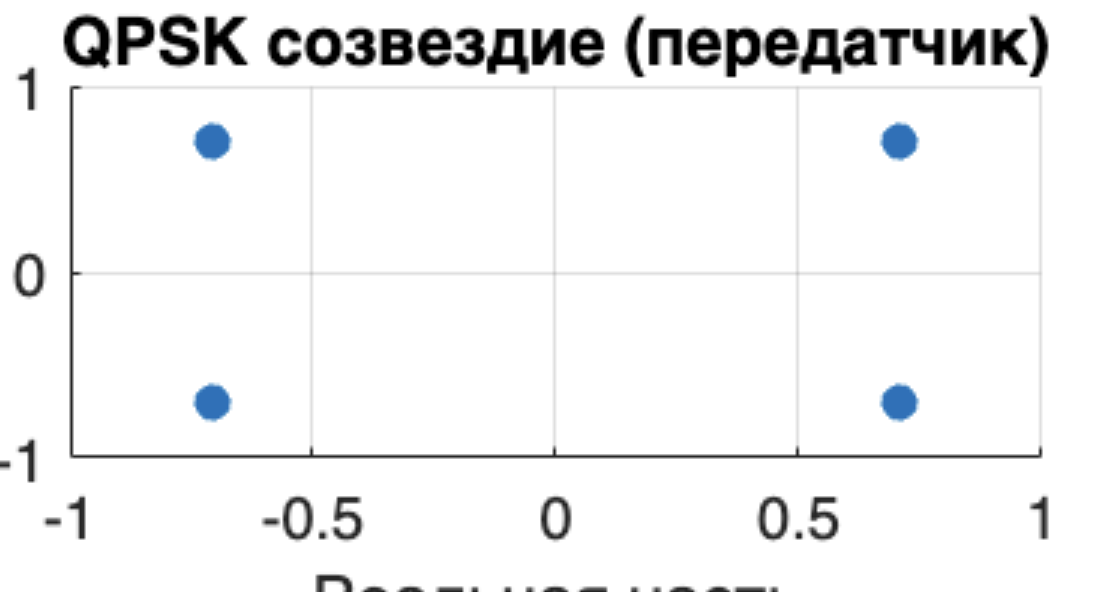
\includegraphics{qpsk_tx.png}
			\caption{QPSK созвездие (передатчик)}
			\label{fig:signal_analysis:d}
		\end{subfigure}
		\hfill
		\begin{subfigure}{0.45\textwidth}
			\centering
			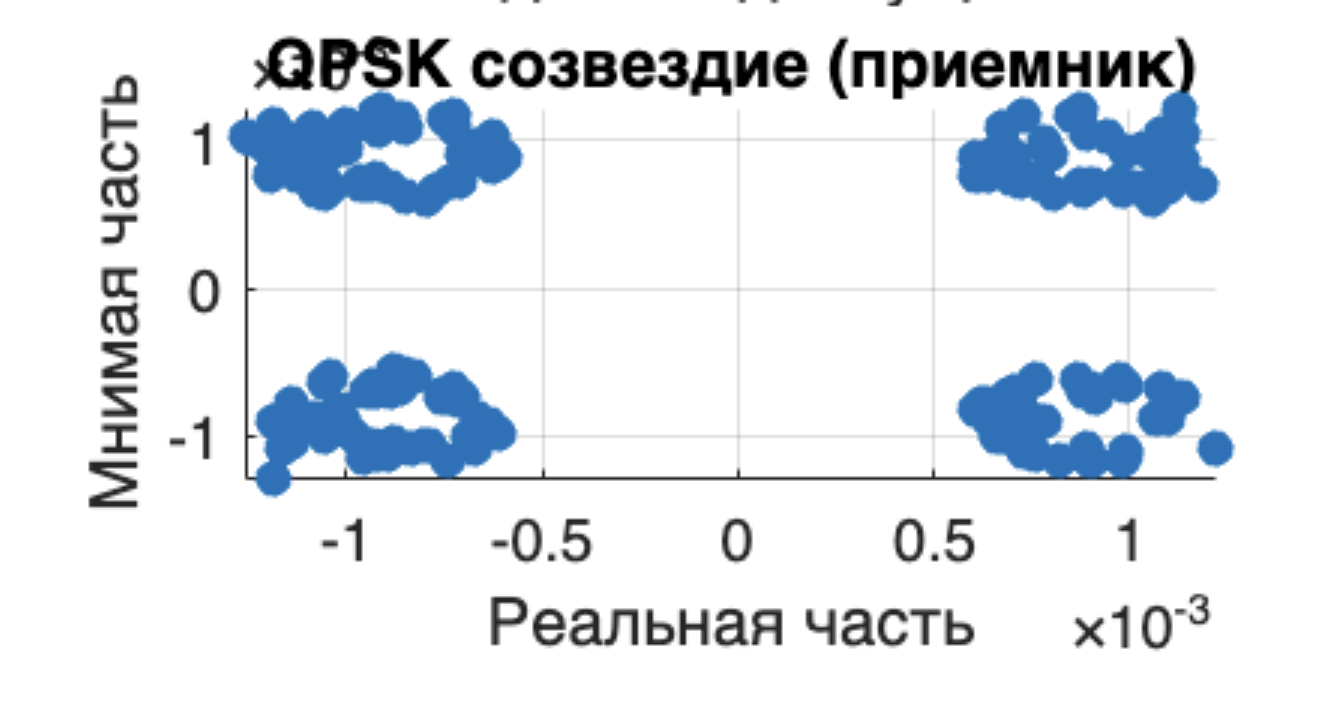
\includegraphics{qpsk_rx.png}
			\caption{QPSK созвездие (приемник)}
			\label{fig:signal_analysis:e}
		\end{subfigure}
		\caption{Графический анализ сигналов}
		\label{fig:signal_analysis}
	\end{figure}
	
	\section{Выводы}
	
	Реализация полного цикла обработки сигнала в OFDM системе показала успешное кодирование, передачу и восстановление сообщения. Моделирование многолучевого канала и добавление шума позволили оценить устойчивость системы. Графический анализ подтвердил корректность модуляции и демодуляции. Дальнейшие исследования могут включать анализ при различных уровнях шума и адаптивную модуляцию.
	
	% Bibliography
	\printbibliography[title=Список использованных источников]
	
\end{document}